\chapter{The Timing Library (.lib): How Cells Tell Time}

\begin{tldr}
\begin{itemize}[leftmargin=*]
  \item \textbf{Last chapter:} a netlist is just a graph of instances, nets, and ports. \textbf{This chapter:} we feed that graph to the timing engine, which only knows what each cell does because the \texttt{.lib} tells it.
  \item A \textbf{.lib} is the Liberty-format file that tells every EDA tool how each standard cell behaves: its pins, function, timing arcs, power, and leakage.
  \item Timing inside a .lib is stored as \textbf{NLDM lookup tables} indexed by \textbf{input slew} and \textbf{output load}; the tool reads the table and \textbf{bilinearly interpolates} when your operating point falls between grid samples.
  \item \textbf{CCS} and \textbf{ECSM} add a third axis (time-varying current) to model Miller capacitance accurately at sub-130\,nm nodes, at the cost of much larger library files.
  \item Foundries deliver one .lib per \textbf{PVT corner} (slow-slow worst case, typical, fast-fast best case); a real flow loads many of them under \textbf{MMMC} so STA can sign off across all corners simultaneously.
  \item Tools compile .lib into a binary \textbf{.db} (Synopsys) for fast ingestion, but engineers always debug against the human-readable .lib.
\end{itemize}
\end{tldr}

\section*{Why this chapter exists}

You hand the place-and-route tool a netlist that says \texttt{INVX1 U7 (.A(n42), .Y(n43));}. The tool stares back and asks a question you cannot answer from the netlist alone: \emph{how long does it take for a transition on n42 to appear on n43?} That number is not in the Verilog. It is not in the library exchange format. It lives in exactly one place, and that place is the timing library. Without it, no static timing analysis runs, no gate sizing happens, no clock tree gets built, and no chip taped out.

\textbf{This chapter unpacks what is actually inside that file.} We will look at a real NLDM lookup table, watch a tool interpolate a delay value step by step, and then see where NLDM breaks down and CCS takes over.

\section{The Two Axes of Cell Delay}

A standard cell's delay is not a constant. It depends on \textbf{how sharp the incoming edge is} (input slew, or \texttt{tran}) and \textbf{how much capacitance the output is driving} (output load, or \texttt{cap}). A slow input edge stretches the delay; a heavy output load stretches it more. Every other gate-level timing question reduces to those two knobs.

The Liberty file captures this by storing a 2D \textbf{lookup table} per timing arc per cell. Rows are discrete input-slew values. Columns are discrete output-load values. Each cell holds a delay (and a separate table holds output slew). When the tool needs a point that is not on the grid, it interpolates.

\subsection*{Figure 1: NLDM delay surface for an INVX1 cell}

\begin{figure}[h]
\centering
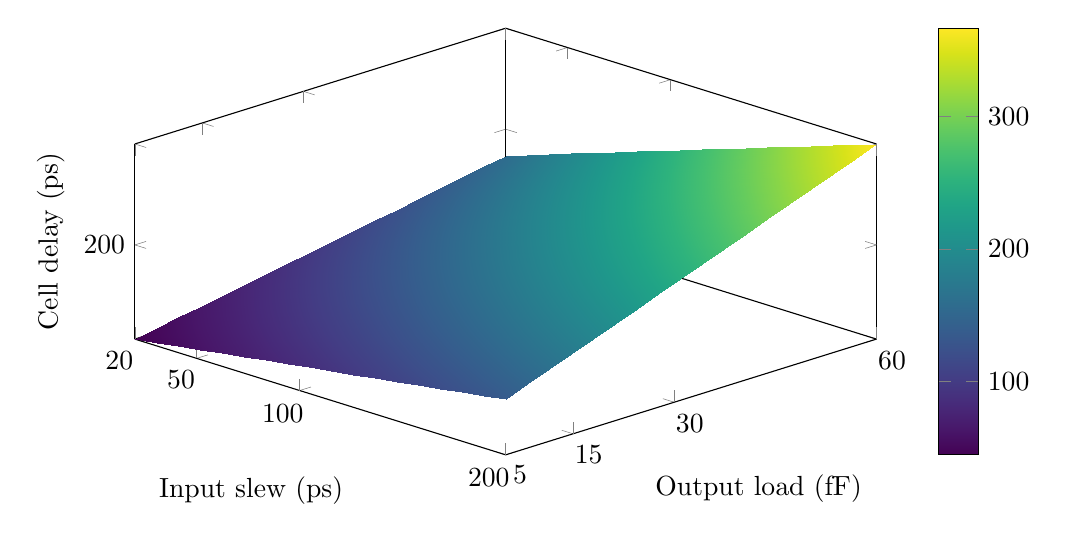
\begin{tikzpicture}
  \begin{axis}[
    width=11cm, height=7cm,
    view={45}{40},
    xlabel={Input slew (ps)},
    ylabel={Output load (fF)},
    zlabel={Cell delay (ps)},
    colormap/viridis, colorbar,
    xtick={20,50,100,200}, ytick={5,15,30,60},
    enlargelimits=false,
  ]
    \addplot3[surf, shader=interp, samples=18, domain=20:200, y domain=5:60]
      {25 + 0.45*x + 1.8*y + 0.012*x*y};
  \end{axis}
\end{tikzpicture}
\caption{NLDM delay surface for a representative INVX1 cell. Delay grows roughly linearly with each axis and faster along the diagonal because the slew and load effects multiply. Real .lib tables sample this surface at \textbf{3 to 7 grid points per axis}.}
\end{figure}

\begin{hook}
\textbf{Hook 1.} \textbf{The fork pierces the steak slowly when the steak is cold.} A cold steak is a heavy load; a dull fork is a slow slew. Both make the bite take longer. Stakes: order the wrong cell drive strength and your hold-time margin evaporates before you can re-spin.
\end{hook}

\begin{hook}
\textbf{Hook 2.} \textbf{The librarian stamps every book at three temperatures.} The .lib is the stamp catalog; the librarian is the foundry; the temperatures are PVT corners. Skip a corner and a chip ships that fails in the Arizona heat. Stakes: an entire wafer lot scrapped.
\end{hook}

\begin{gut}
\textbf{Gut check 1.} If you double the output load but keep input slew fixed, what happens to cell delay in an NLDM model?
\gutans{It grows, but not linearly in general. The lookup table captures whatever curvature the SPICE characterization measured. For an INVX1 on a typical 28\,nm node, doubling load from 15\,fF to 30\,fF might raise delay by roughly 60 to 80 percent.}
\end{gut}

\begin{gut}
\textbf{Gut check 2.} Why does the .lib store \emph{two} tables (rise and fall) per timing arc instead of one?
\gutans{NMOS and PMOS have different mobilities. The pull-down path through NMOS is usually faster than the pull-up through PMOS, so rise and fall delays differ. The tool needs both to compute setup and hold against the correct edge.}
\end{gut}

\begin{pausebox}
So far: a .lib is the file that tells the tool how a cell delays a signal, the delay depends on input slew and output load, and the data is stored as a 2D table per arc per cell. Next: we read a real Liberty snippet and then do the arithmetic the tool does.
\end{pausebox}

\begin{keyidea}
A timing library is a \textbf{characterized lookup of cell behavior across PVT corners}. The NLDM model boils every cell's delay down to a 2D table indexed by input slew and output load, and the tool interpolates between grid points whenever your operating condition falls in between.
\end{keyidea}

\section{What a Liberty File Actually Looks Like}

\subsection*{Figure 2: A real Liberty timing block for an inverter}

\begin{lstlisting}[style=eda, language=, caption={Excerpt of an INVX1 cell in Liberty format. The \texttt{lu\_table\_template} (defined once at the top of the .lib) declares the index variables; each \texttt{cell\_rise} / \texttt{cell\_fall} group fills in the delay surface for one timing arc.}]
library (tsmc28_tt_0p9v_25c) {
  time_unit              : "1ns";
  capacitive_load_unit (1, ff);
  voltage_unit           : "1V";
  nom_voltage            : 0.90;
  nom_temperature        : 25.0;

  lu_table_template (delay_template_3x3) {
    variable_1 : input_net_transition;
    variable_2 : total_output_net_capacitance;
    index_1 ("20.0, 100.0, 200.0");   /* ps */
    index_2 ("5.0,  15.0,  30.0");    /* fF */
  }

  cell (INVX1) {
    area : 1.764;
    pin (A) { direction : input;  capacitance : 1.42; }
    pin (Y) {
      direction : output;
      function  : "!A";
      max_capacitance : 60.0;
      timing () {
        related_pin   : "A";
        timing_sense  : negative_unate;
        cell_rise (delay_template_3x3) {
          values ( "0.045, 0.062, 0.091", \
                   "0.071, 0.094, 0.135", \
                   "0.108, 0.142, 0.198" );
        }
        cell_fall (delay_template_3x3) {
          values ( "0.038, 0.054, 0.080", \
                   "0.061, 0.083, 0.121", \
                   "0.094, 0.127, 0.178" );
        }
      }
    }
  }
}
\end{lstlisting}

Two things deserve attention in that listing. First, the \textbf{units block at the top} sets the scale for every number below: delays are in \texttt{ns}, capacitances in \texttt{fF}. Misreading the unit is the single most common .lib bug junior engineers commit. Second, the \textbf{values} array is row-major, with rows indexed by \texttt{index\_1} (input slew) and columns by \texttt{index\_2} (output load).

\section{Worked Example: Bilinear Interpolation by Hand}

Let us take the \texttt{cell\_rise} table from the listing above and ask: what is the cell delay if the input slew is \textbf{50\,ps} and the output load is \textbf{15\,fF}? The exact load (15\,fF) sits on the grid, but the slew (50\,ps) falls between 20\,ps and 100\,ps, so we have to interpolate along one axis.

\textbf{Step 1: locate the bracketing grid points.} Slew 50\,ps lies between \texttt{index\_1[0]=20} and \texttt{index\_1[1]=100}. Load 15\,fF is exactly \texttt{index\_2[1]=15}.

\textbf{Step 2: pull the four corner delays.} Because load sits on the grid, only two corners matter:
\[
D(20\,\text{ps},\,15\,\text{fF}) = 0.062\,\text{ns}, \qquad D(100\,\text{ps},\,15\,\text{fF}) = 0.094\,\text{ns}.
\]

\textbf{Step 3: compute the slew fraction.}
\[
\alpha = \frac{50 - 20}{100 - 20} = \frac{30}{80} = 0.375.
\]

\textbf{Step 4: linearly blend.}
\[
D_{\text{interp}} = (1 - 0.375)\cdot 0.062 + 0.375 \cdot 0.094 = 0.625 \cdot 0.062 + 0.375 \cdot 0.094.
\]
\[
D_{\text{interp}} = 0.03875 + 0.03525 = 0.0740\,\text{ns} = \mathbf{74.0\,ps}.
\]

So the tool reports a rise delay of \textbf{74\,ps} for this INVX1 under those conditions. Now let us do the harder case where \emph{both} axes are off-grid: slew 50\,ps, load 22\,fF.

\move{1} Pull all four corners:
\[
\begin{aligned}
D_{00} &= D(20, 15) = 0.062, & D_{01} &= D(20, 30) = 0.091,\\
D_{10} &= D(100, 15) = 0.094, & D_{11} &= D(100, 30) = 0.135.
\end{aligned}
\]

\move{2} Compute fractions on each axis:
\[
\alpha = \tfrac{50-20}{100-20} = 0.375, \qquad \beta = \tfrac{22-15}{30-15} = \tfrac{7}{15} = 0.4667.
\]

\move{3} Interpolate along load at each slew value:
\[
D(20, 22) = (1-0.4667)\cdot 0.062 + 0.4667 \cdot 0.091 = 0.0331 + 0.0425 = 0.0756.
\]
\[
D(100, 22) = (1-0.4667)\cdot 0.094 + 0.4667 \cdot 0.135 = 0.0501 + 0.0630 = 0.1131.
\]

\move{4} Interpolate the two intermediate values along slew:
\[
D = (1-0.375)\cdot 0.0756 + 0.375 \cdot 0.1131 = 0.0473 + 0.0424 = \mathbf{0.0897\,\text{ns}} \approx \mathbf{90\,ps}.
\]

\move{5} Generalize to the abstract \textbf{bilinear interpolation formula}:
\[
D(s, c) = (1-\alpha)(1-\beta)\,D_{00} + \alpha(1-\beta)\,D_{10} + (1-\alpha)\beta\,D_{01} + \alpha\beta\,D_{11}
\]
where \(\alpha\) is the fractional position along input slew and \(\beta\) is the fractional position along output load. The hand arithmetic above is exactly this formula, executed in two passes.

\section{Setup, Hold, and the Other Tables}

NLDM does more than store cell delays. Every sequential cell (flip-flops, latches) carries additional 2D tables that encode timing checks: a \textbf{setup} table indexed by data-slew and clock-slew, and a \textbf{hold} table with the same axes. The tool reads these to determine whether captured data is stable around the active clock edge. There are also \textbf{recovery} and \textbf{removal} tables for asynchronous pins, and \textbf{output transition} tables that propagate the slew downstream so the next gate's delay table can be looked up correctly.

\begin{pitfall}
\textbf{Watch Out.}
\begin{itemize}[leftmargin=*]
  \item \textbf{Units are not universal.} One foundry's .lib uses \texttt{1ns} and \texttt{pF}; another uses \texttt{1ps} and \texttt{fF}. Mixing tools that disagree on the units block produces silent errors of 1000x.
  \item \textbf{NLDM is not CCS.} Reading a .lib that claims CCS support but only filling in NLDM tables gives you NLDM accuracy with CCS file size. Verify by grepping for \texttt{output\_current\_rise}.
  \item \textbf{Hold tables are not setup tables.} A common bug: copying setup characterization data into the hold slot. Setup and hold have opposite signs and different reference edges.
  \item \textbf{PVT corners are not interchangeable.} The slow-slow (\textbf{WC}) .lib is for setup analysis; the fast-fast (\textbf{BC}) .lib is for hold. Loading only the typical (TC) corner will sign off a chip that fails silicon.
\end{itemize}
\end{pitfall}

\section{Why CCS Exists (and Why NLDM Quietly Lies at 7nm)}

NLDM stores \textbf{one delay number} per (input slew, output load) grid point. That model rests on three assumptions, and every single one of them gets shakier as nodes shrink.

\textbf{Assumption 1: the output load is a fixed lumped capacitor.} It is not. Gate-to-drain coupling capacitance (the \textbf{Miller capacitance}) at the receiver gets multiplied by $(1 + A_v)$ where $A_v$ is the receiver's small-signal gain during the transition. In a fast switching transition the effective load the driver feels is meaningfully larger than the static fanout capacitance the .lib was characterized against.

\textbf{Assumption 2: the receiver's input pin capacitance is constant.} It is not. PMOS and NMOS gate capacitance is voltage-dependent: a gate in cutoff presents less capacitance than the same gate in saturation. As the input ramps, the load looks different at 30\% Vdd than at 70\% Vdd. NLDM averages this and ships one number per pin. CCS stores the nonlinearity.

\textbf{Assumption 3: only the slew (20\%-to-80\% or similar) matters, not the waveform shape.} At 130\,nm a slew was a clean, near-linear ramp. At 7\,nm the upstream driver's output is non-monotonic enough that two transitions with the same 20-80 slew can produce \textbf{different downstream delays}. NLDM cannot see this. CCS can, because it propagates the actual current waveform.

\begin{keyidea}
CCS replaces NLDM's single delay number with a \textbf{time-varying output current waveform per (slew, load) grid point}, so the next stage convolves \emph{actual current shape} into its own response instead of inheriting a slew-only summary.
\end{keyidea}

\paragraph{Worked example: when NLDM and CCS diverge.} A buffer drives a fanout-of-4 load. NLDM says: static load = 4 input gates $\times$ 1.0\,fF = 4.0\,fF, look up (slew = 50 ps, load = 4 fF) in the table, get \textbf{delay = 32 ps}. CCS sees that the receiver's effective Miller-multiplied capacitance during the transition is closer to $4.0 \times 1.4 = 5.6$\,fF, AND that the receiver pin cap rises by ~20\% as the input crosses the switching threshold. The CCS-computed delay is \textbf{closer to 42 ps}. \textbf{A 30\% error on a single stage, compounded over a 15-stage path, is the difference between meeting timing and missing it by 100\,ps.}

\textbf{ECSM} (Cadence) encodes the same physics with a voltage-vs-time waveform instead of current-vs-time. Same intent, different storage. Innovus consumes ECSM natively; PrimeTime consumes CCS. Foundries ship both.

\textbf{File size cost.} A CCS .lib is roughly 5 to 10x the size of the equivalent NLDM library because every (slew, load) entry now stores a sampled current waveform (typically 20 time points) instead of one delay scalar. This is why the .db (binary compiled .lib) matters: loading 200 CCS views as ASCII text would burn an hour on Liberty parsing alone.

\begin{sidebar}
\textbf{Why MMMC makes this worse.} CCS file size multiplied by MMMC view count is what actually fills your scratch disk. A 5\,nm block with 200 .lib views, each in CCS form at ~80\,MB, lands at ~16\,GB of library data per run. The binary .db form compresses this maybe 3x. \textbf{This is why the LIBPATH variable in Innovus matters and why corrupted .db caches eat days.}
\end{sidebar}

\begin{pdnote}
\begin{itemize}[leftmargin=*]
  \item \textbf{Arm internship lens.} When a designer hands you a failing path, the first reflex is to open the .lib for the offending cell and confirm its drive strength, max-cap, and the actual delay numbers at the path's slew and load. Half the bugs assigned to junior PD engineers turn out to be a misloaded corner library.
  \item \textbf{Foundry-flow PD engineer lens.} You will routinely load \textbf{8 to 32 libraries} per run under MMMC: WC, TC, BC across two voltage rails and three temperatures, times functional mode (sleep, active, scan). Knowing which corner pessimizes setup vs hold determines which library a slack violation belongs to and where the fix has to land.
  \item \textbf{VLSI interview lens.} Expect \emph{"walk me through what's inside a .lib file"} and \emph{"why CCS over NLDM at advanced nodes?"} as warm-up questions. The strong answer names the units block, the lookup template, the timing arc with related\_pin and timing\_sense, and finishes with Miller capacitance and receiver-pin modeling as the CCS justification.
\end{itemize}
\end{pdnote}

\begin{checkpoint}
You can now (1) name the four things a .lib stores per cell (pins, function, timing arcs, power), (2) read an NLDM lookup table and bilinearly interpolate a delay by hand, (3) explain why CCS exists and what it adds, and (4) defend why a real flow loads many .lib files under MMMC rather than just one.

\mnemonic{Slew in, load out, table in the middle, corner on the side.}
\end{checkpoint}
